\chapter{Direct communication}

\section{Introduction}


\subsection{Data representation}

\emph{Marshalling} is the assembling of a collection of data items into a form suitable for transmission, whereas \emph{unmarshalling} is the disassembling of a message on arrival to produce the equivalent collection of data items. For example Java uses serialization and deserialization of objects, or SOAP in Service Oriented Architectures et cetera [2].


\subsection{Message passing}

\textbf{Table 1} lists the two basic operations in message passing.

\begin{table}
	\caption{Basic message passing API.}
	\label{tab:}
	\begin{tabular}{p{150px} | p{250px}}
		\textbf{Operation} & \textbf{Description} \\
		\hline
		send (p: PortId; m: Message) & Send a message \emph{Message} to a process at a port with given \emph{PortId}. \\
		receive (p: PortId; VAR m: Message) & Receive a message \emph{Message} while listening at a port with given \emph{PortId}. \\
		\hline
	\end{tabular}
\end{table}


The semantics of send and receive operations can differ. In \emph{synchronous} send the process waits for the corresponding receive. In synchronous receive, the process waits for the message arrival. In \emph{asynchronous} send the process does not wait for the message arrival. In aynschronous receive, the process announces its willingness to accept or check for message arrival [2].

There a various possible message destinations, e.g., \emph{processes}, which have a single entry point per process for all messages, or \emph{ports}, which have one receiver and possibly many senders, or \emph{mailboxes}, which may have many receivers [2].


\subsubsection{Reliable communication}

Failures in message passing may be the result of a number of causes, for example corrupted messages, duplicate messages, omission, i.e., the loss of messages, wrong ordering of messages, or receiver process failures [2]. In order to achieve reliable communication, messages should be delivered uncorrupted, in order, without duplicates, despite a reasonable number of packets dropped or lost. Unfortunately perfectly reliable communication can not often be guaranteed [2].

Reliable communication can be implemented using a number of techniques, for example [2]:
\begin{itemize}
	\item \textbf{Corruption} : Include checksum in message;
	\item \textbf{Order mistakes and duplicates} : Include a message number which identifies the message;
	\item \textbf{Omission} : Sender stores message in buffer, sends it and sets a time-out and the receiver replies with acknowledgement. If no aknowledgement was received, the sender retransmits messages after timeout.
\end{itemize}



\section{Remote invocation}

\subsection{Request-reply protocols}

Request-reply protocols are designed to support roles and message exchanges in typical client-server interactions. \textbf{Table 2} lists the basic operations of request-reply protocols. \textbf{Figure 1} shows the general model for request-reply protocols.


\begin{table}
	\caption{Basic request-reply protocol operations.}
	\label{tab:}
	\begin{tabular}{p{150px} | p{250px}}
		\textbf{Operation} & \textbf{Description} \\
		\hline
		doOperation		& The client sends request and returns answer to the application program. \\
		getRequest		& The server gets the request from the client. \\
		sendReply			& The server sends a reply to the client. \\
		\hline
	\end{tabular}
\end{table}


\begin{figure}
	\begin{center}
		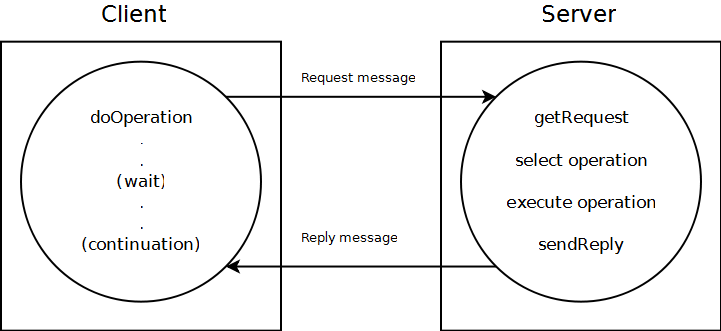
\includegraphics[width=0.7\textwidth]{img/requestreplycommunication}
	\end{center}
	\caption{Model for request-reply communication.}
	\label{fig:requestreplycommunication}
\end{figure}



\subsubsection{Reliable communication}

In reliability measures of TCP are an overkill as the acknowledgement from the receiver is redundant because the reply message is an acknowledgement. As a result, UDP can be used for building more efficient client server communication [2].



\subsection{Remote procedure call}

Traditional applications consist of a main program with a number of procedures (functions). In distributed systems procedures are grouped into servers, and main programs become clients. To achieve transparency the (remote) operations on a server from a client should look like conventional procedure calls [2].

To achieve this an additional message subsystem is introduced. When an application program calls client \emph{stub procedure}, the client stub procedure marshalls parameters of call and gives it to \emph{communication module} in client. The communication module then transmits a message with the marshalled RPC to the server's communication module who passes it on to the \emph{dispatcher}. The dispatcher determines which procedure is called and calls the correct server stub procedure. Next, the server stub procedure unmarshalls data and calls the relevant server procedure. The server procedure returns the answer to the server stub procedure. The result is marshalled and sent to the client via the communication modules. The communication module at client side gives data to client stub procedure, who finally unmarshalls data and returns the answer to the calling program [2]. \textbf{Figure 2} shows the architectural elements in this scenario.


\begin{figure}
	\begin{center}
		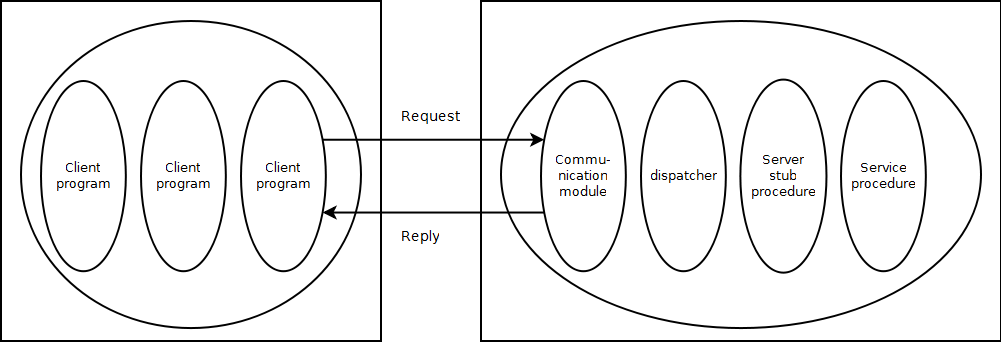
\includegraphics[width=0.7\textwidth]{img/rpc}
	\end{center}
	\caption{Remote procedure call.}
	\label{fig:rpc}
\end{figure}

\emph{Remote procedure calls} (RPC) can be integrated within a particular programming language, or based on a special \emph{interface definition language} (IDL) [2].


\subsubsection{Design issues}

\paragraph{Heterogeous environment}

An Interface Definition Language (IDL) tries to provide abstraction for the heterogeneity of client and server implementations through programming language-independency. IDL describes operation signatures and its interface compilers are used as a base for generating client and server stubs, which can be implemented in different languages [2].


\paragraph{Transparancy}

To achieve transparency, RPC should be as much like local procedure calls as possible. However the calling instruction set is different, and there is no shared memory between caller and callee [2].

RPC requires some form of exception handling as failures cannot be hidden. Clients cannot distinguish between network failures or server failures. To deal with failures, language specific solutions may be applied, expressive return codes of functions, or extensions provided by IDL [2].

\paragraph{Semantics}


Remote procedure calls may have the following semantics [2]:
\begin{itemize}
	\item \textbf{Maybe} : Requests are not resent, as a result no duplicate filtering is required, and it logically follows that procedure need no re-exececution, and no replies are re-transmited;
	\item \textbf{At-least-once} : Requests are re-sent, but as there is no duplicate filtering, procedures can be re-exececuted. To retain system consistency, operations have to be idempotent;
	\item \textbf{At-most-once} : Requests are re-sent, hence duplicate filtering is required and replies are re-transmitted. Procedures can not be re-exececuted;
	\item \textbf{Exactly-once} : Difficult or impossible given failures;
\end{itemize}



\subsubsection{Implementation aspects}

The task of the interface compiler is to generate client and server stub procedures, marshalling and unmarshalling operations for each argument type, and implement headers for server procedures.

Binding is the linking of the client to the server at execution time: the server will register a service at binder, and the client will perform a lookup for the service. Locating the binder is done through a well-known host address and is the responsibility of the operating system [2].


\subsubsection{Asynchronous RPC}

Asynchronous RPC can be used to reduce the idle time of processes that are waiting for a remote procedure call to complete [2].



\subsubsection{Conclusions}

RPC is a familiar paradigm which has been a basic primitive for distributed programming for many applications and systems [2].

RPC has some limitations with respect to failure handling, no transaction support, and the fact that RPC only supports one-to-one communication [2].



\subsection{Remote method invocation}

\emph{Remote method invocation} (RMI) is a technology that similar to RPC allows clients to invoke methods on remote objects. It also uses programming with interfaces, called \emph{remote interfaces}, can offer a number of call semantics and provides a similar level of transparancy as RPC, i.e., local and remote calls have the same syntax but the distributed nature of calls can be exposed, e.g., through remote exceptions. As a result, they share many of the design issues explained earlier, with the additional design issue of dealing with (distributed) objects for RMI [1].

RMI allows parameter passing by value, as input or output parameters, and also as object references. Remote invocation can then be used on these object references, instead of transmitting the complete object value accross the network [1]. The possible remote invocations are listed in the remote interface of that object.


\subsubsection{Distributed objects}

\paragraph{Classic object model}

Objects are accessed via their reference. An object is associated with an interface, which separates the method signatures from the actual implementation. Actions in object-oriented programs are initiated by invoking a method in another object [1]. Three possible effects are associated with method invocation [1]:
\begin{enumerate}
	\item Change of the target object state, which consists of the values of its instance variables;
	\item Creation of a new object;
	\item Resulting in a new invocation on methods in other objects.
\end{enumerate}
To deal with errors during execution, exceptions are used to create clearer error handling in complex code. Exceptions are a way to alter the control flow of a program [1].

A garbage collector detects when objects are no longer used and frees the memory occupied by these instances.

\paragraph{Distributed object model}

\emph{Distributed objects} are objects that are managed by a server and implement a \emph{remote interface} by which clients can invoke on the distributed object via its \emph{remote object reference}. A remote object reference is an identifier that can be used throughout the distributed system to refer to a unique remote object [1].

\emph{Remote exceptions} reveal some of distributed nature of RMI. Aside from errors in the program, exceptions in remote objects may be due to crashes in the server process, timeouts due to network failure et cetera [1].

In a distributed context, distributed garbage collection is slightly more complicated as object references may be spread accross different machines. It is achieved by extending the local garbage collection with a distributed module, often based on reference counting [1].


\subsubsection{RMI implementation}

\textbf{Figure 3} shows the remote method invocation architectural components. In what follows we describe some of these components in more detail to finally form the complete picture of the RMI technology.

\begin{figure}
	\begin{center}
		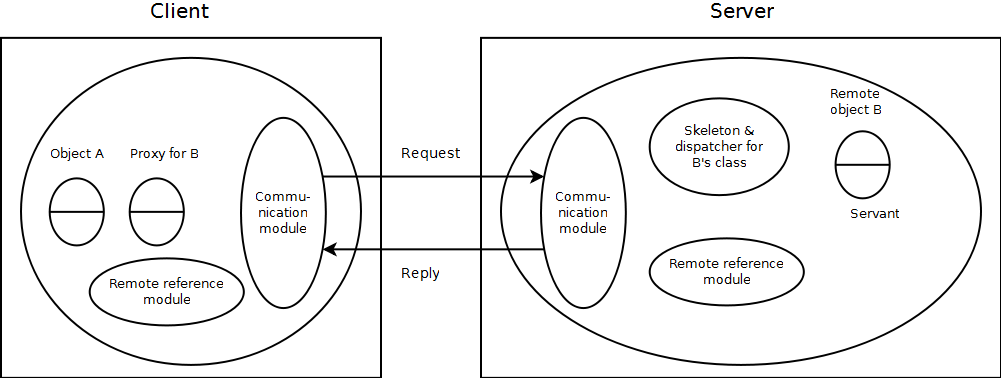
\includegraphics[width=0.7\textwidth]{img/rmi}
	\end{center}
	\caption{Remote method invocation.}
	\label{fig:rmi}
\end{figure}


\paragraph{Communication module}

Communication modules operate using a request-reply protocol between client and server. They are responsible for enforcing specific invocation semantics, e.g., \textit{at-most-once} [1].

When a request is received by the server's communication module, the communication module passes on the remote reference in the request to the remote reference module which returns the local reference. Next the server's communication module selects the dispatcher for the class of the object to be invoked (cf. RPC), passing on the local reference [1].


\paragraph{Remote reference module}

The task of the \emph{remote reference module} is to translate between remote and local references by looking them up in a \emph{remote object table}. The remote object table holds the following information [1]:
\begin{itemize}
	\item Each remote object held by the process at the server's remote reference module;
	\item Each local proxy at the client's remote reference module.
\end{itemize}


\paragraph{RMI software layer}

The \emph{RMI software layer} is a layer between the application-level objects and the communication and remote reference modules. The following middleware components are part of this layer [1]:

\begin{itemize}
	\item \textbf{Proxy} : The proxy appears as a normal object in the client process, achieving some transparancy. However, instead of executing invocations, it forwards them in a message to the corresponding remote object after marshalling arguments. Results from the invocation are then unmarshalled and passed on to the client process;
	\item \textbf{Dispatcher} : For each class representing a remote object there is one skeleton and one dispatcher at the server. The dispatcher receives requests from the communication module;
	\item \textbf{Skeleton} : The class of a remote object has a skeleton, which implements the methods in the remote interface. It is responsible for marshalling and unmarshalling arguments and results respectively of requests before passing them on to the servant. A \emph{servant} is an instance of a class that provides the body to a remote object. Servants live within a server process and handles the remote requests passed on by the corresponding skeleton;
\end{itemize}




\section*{References}

\begin{enumerate}[1]
	\item G. Coulouris, J. Dollimore, T. Kindberg and G. Blair, "Distributed Systems: Concepts and Design (5th Edition)", M. Horton, Red., Addison-Wesley, 2011, p. 1063.
	\item W. Joosen, 2013, "Distributed Systems Direct Communication PART I", iMinds-DistriNet, KULeuven
	\item W. Joosen, 2013, "Distributed Systems Direct Communication PART II", iMinds-DistriNet, KULeuven
\end{enumerate}